\subsection{The notion of a quantum state}

A quantum state represented by a positive Hermitian operator $\hat{\rho}$ with unit trace, contains all physically relevant information about a quantum system. If two quantum systems are prepared in identical states, any measurement performed on them will yield identical outcome probabilities, making the different preparation methods observationally equivalent. Conversely, if the systems are in different quantum states, there necessarily exists at least one measurement that produces different probability distributions, allowing their preparations to be distinguished. The systematic process of designing and performing measurements to identify which of several possible states (and thus which preparation) a given system is in is called quantum state discrimination. 

\subsection{Measuring a quantum state}

While the quantum state itself is an abstract mathematical object, measurements provide it with concrete operational meaning. The outcomes of quantum measurements are always classical, such as a photodetector click count or an ion’s position in a trap, and these outcomes behave as random variables. By performing the same measurement many times on identically prepared quantum systems, one can reconstruct the statistical distribution of outcomes. If this process is repeated for every possible measurement, the complete set of outcome probability distributions fully characterizes the quantum state. Thus, the state is not directly observable, but its empirical reality is revealed through the statistics of measurement outcomes, bridging the gap between abstract formalism and experimental practice. The formal relationship between quantum states and measurements is captured by the postulates of standard quantum measurement theory. These postulates can be summarized as follows:

\begin{enumerate}
    \item Every physical observable corresponds to a Hermitian operator $\hat{X}$ with a spectral decomposition
    \begin{equation}
        \hat{X} = \sum_j \lambda_j |j\rangle\langle j|
    \end{equation}
    where $\lambda_j$ are the possible measurement outcomes.

    \item The projectors 
    \begin{equation}
        P_j = |j\rangle\langle j|
    \end{equation}
     associated with the eigenstates form a complete set, satisfying 
     \begin{equation}
         \sum_j P_j = \mathbb{I}
     \end{equation} and are orthogonal such that 
     \begin{equation}
         P_i P_j = \delta_{ij} P_i
     \end{equation}
     
    \item A measurement of $\hat{X}$ yields one of its eigenvalues $\lambda_j$ as the result.

    \item If the outcome $\lambda_j$ is obtained, the system collapses to the post-measurement state 
    \begin{equation}
        \hat{\rho}_j = \frac{P_j \hat{\rho} P_j}{\operatorname{tr}(P_j \hat{\rho} P_j)}
    \end{equation}

    \item The probability of obtaining the outcome $\lambda_j$ is given by 
    \begin{equation}
    p_j = \operatorname{tr}(\hat{\rho} P_j)    
    \end{equation}
    
    \item When the measurement is performed but the outcome is not recorded, the post-measurement state is described by the density operator 
    \begin{equation}
        \hat{\rho}' = \sum_j P_j \hat{\rho} P_j
    \end{equation}
     representing an average over all possible outcomes.
\end{enumerate}

It is important to note that in stating the postulates, the Hilbert space has been assumed to be finite and discrete solely for the sake of notational simplicity. In principle, these postulates apply equally to states with infinite-dimensional Hilbert spaces, which is precisely the case for continuous variable systems. The postulates make it clear that the measurement process is fundamentally random, with the outcome able to take a range of values. The number of possible measurement outcomes is equal to the dimension of the Hilbert space of the state. The projection operators $P_j$ used in this formulation are referred to as projective measurements or von Neumann measurements. However, it turns out that the requirement that measurement operators be strictly projective can be relaxed while still maintaining a meaningful statistical distribution for the outcomes. In particular, Postulate 3 provides an algorithm for generating outcome probabilities. \\

If we replace the projective measurement operator $P_j$ with a positive operator $\Pi_j$ that may not necessarily be a projection, the probability of obtaining outcome $j$ is given by 
\begin{equation}
    p_j = \operatorname{tr}(\hat{\rho} \Pi_j)
\end{equation}
 Since $\Pi_j$ is a positive operator, $p_j \geq 0$, and if we further require that the set of such operators for a finite set of outcomes is complete, meaning $\sum_j \Pi_j = \mathbb{I}$, then the quantities $p_j$ can be interpreted as probabilities for the outcomes of the measurement described by the operator set $\{\Pi_j\}$. Such a set of measurement operators is called a positive operator valued measure, or POVM. A key feature of POVMs is that their elements do not need to be orthogonal. Consequently, the number of possible outcomes can be larger than the dimension of the Hilbert space of the state being measured, offering greater flexibility in measurement design.\\

 Using POVMs, we can replace the postulates of the quantum theory of standard measurements with the following more flexible ones:

\begin{enumerate}
    \item Measurement operators are positive operators $\Pi_j \geq 0$ where the set of all such operators is complete: $\sum_j \Pi_j = \mathbb{I}$. The set of such operators is called a POVM. The elements of the POVM can be written in terms of generalized measurement operators $A_j$, where 
    \begin{equation}
        \Pi_j = A_j^\dagger A_j
    \end{equation}
     The generalized measurement operators can be non-Hermitian, though the elements of the POVM must be Hermitian by construction.
    
    \item Each element of the POVM set represents a possible outcome of the measurement.
    
    \item The state of the system after the measurement is
    \begin{equation}
    \hat{\rho}_j = \frac{A_j \hat{\rho} A_j^\dagger}{\operatorname{tr}(A_j \hat{\rho} A_j^\dagger)}    
    \end{equation}

    
    \item The probability that the outcome $j$ (indexing the measurement operator $\Pi_j$) is found is 
    \begin{equation}
    p_j = \operatorname{tr}(\Pi_j \hat{\rho})    
    \end{equation}
    
    
    \item If we perform the measurement but do not record the results, the post-measurement state is described by the density operator 
    \begin{equation}
    \hat{\rho}' = \sum_j A_j \hat{\rho} A_j^\dagger    
    \end{equation}
    
\end{enumerate}

The POVM formalism described above provides a way to describe classical information obtained from a quantum state by way of a measurement. State discrimination is the process of processing this information to determine, to the best of our knowledge, which quantum state we possess. The fundamental question of how well we can discriminate between quantum states lies at the heart of quantum mechanics. When the set of possible states are orthogonal to one another, perfect discrimination is always possible. This can be achieved by choosing a set of projection operators that correspond exactly to the set of possible states. However, when the possible states are non-orthogonal, perfect discrimination is impossible. In such cases, we must define optimal discrimination with respect to some figure of merit, though finding this optimal discrimination is often non-trivial. The chapter will next set up the problem of state discrimination and describe two commonly used strategies: minimum-error discrimination and unambiguous discrimination. Following that, some interesting well-known measurements that do not fall into these two categories, such as the pretty-good measurement and the no-measurement strategy, will be discussed.

\subsection{State Discrimination}
Consider an ensemble of quantum systems such that each system is prepared in one of $N$ possible states, say $\hat{\rho}_1, \ldots, \hat{\rho}_N$, with a priori probabilities $p_1, \ldots, p_N$ respectively, where $\sum_{j=1}^N p_j = 1$. In general, the states can be pure or mixed, and they can be either discrete variable states or continuous variable states. The observer performing state discrimination has full knowledge of the ensemble being prepared, meaning he knows the possible states and their prior probabilities. However, he does not know which one of the $N$ states he possesses, and he must make a measurement to determine this. State discrimination describes how he should design and perform these measurements to optimally identify the unknown state.\\

There are two commonly used strategies for state discrimination. The first is discrimination with minimum error, attributed to Helstrom, who studied distinguishing between two given quantum states. Helstrom found an optimum measurement strategy for both mixed and pure states that minimizes the probability of error. This optimum measurement strategy is known as the Helstrom measurement, and the resulting minimum error is called the Helstrom bound. The general problem of discriminating between $N>2$ states with minimum error is considerably more difficult. Although the necessary and sufficient conditions for an optimal measurement have been found, how to implement such an optimal measurement remains an open problem, except for a few special cases.\\

The second strategy is unambiguous discrimination, first proposed by Ivanovic. This strategy allows perfect discrimination between two non-orthogonal states, but with the caveat that a non-conclusive (inconclusive) answer is permitted. The specific case of discriminating between two pure non-orthogonal states was solved by Dieks and Peres. However, the general case of unambiguously discriminating between $N$ pure states remains an open problem. It has been shown by Chefles that unambiguous discrimination is only possible if the states to be distinguished are linearly independent. Additionally, there are active research areas focused on extending unambiguous discrimination strategies to mixed states.\\

Having described the two strategies briefly, let us now discuss each of them in more detail.

\subsubsection{State Discrimination with Minimum Error}
In the minimum error discrimination strategy, we always reach a conclusion about which state was prepared, though errors in this conclusion are inevitable. The goal of the optimal strategy is to minimize the detection error. To formulate this as a definite optimization problem, we must define what constitutes a detection error. \\

Let $\Pi_j$ be the POVM element corresponding to the state $\hat{\rho}_j$ being prepared. According to the postulates of quantum measurement theory, if the actual prepared state is $\hat{\rho}$, the probability of guessing that the state is $\hat{\rho}_j$ is $\operatorname{tr}(\hat{\rho} \Pi_j)$. Since the state $\hat{\rho}_j$ occurs with a priori probability $p_j$, the overall probability of a correct guess is given by 
\begin{equation}
    P_{\text{corr}} = \sum_{j=1}^N p_j \operatorname{tr}(\hat{\rho}_j \Pi_j)
\end{equation}
The detection error is then defined as 
\begin{equation}
    P_{\text{err}} = 1 - P_{\text{corr}}
\end{equation}
To minimize the error, we must minimize $P_{\text{err}}$ over all possible sets of POVM elements $\{\Pi_j\}$ for $j = 1, \ldots, N$ subject to the constraints $\Pi_j \geq 0$ and $\sum_{j=1}^N \Pi_j = \mathbb{I}$. The POVM that achieves this minimization is called the optimal measurement, and the resulting error is the minimum error. The special case of distinguishing single copies of two mixed states will be derived later in Section 3.3.1.

\subsubsection{Unambiguous State Discrimination}
Unlike discrimination with minimum error, in unambiguous discrimination we are not permitted to make measurement errors. However, this strategy does not succeed 100\% of the time, and this trade-off is necessary to achieve error-free discrimination.\\

To illustrate how unambiguous state discrimination works, we consider a simple example involving two pure states $|\psi_0\rangle$ and $|\psi_1\rangle$ occurring with equal a priori probabilities, given by

\begin{equation}
    |\psi_0\rangle = \cos\theta |0\rangle + \sin\theta |1\rangle
\end{equation}
\begin{equation}
    |\psi_1\rangle = \cos\theta |0\rangle - \sin\theta |1\rangle
\end{equation}

These states are non-orthogonal with overlap $\langle\psi_0|\psi_1\rangle = \cos^2\theta - \sin^2\theta = \cos(2\theta)$.\\

A POVM for distinguishing between these states can be constructed with elements

\begin{equation}
    \Pi_0 = a_0(\sin\theta |0\rangle + \cos\theta |1\rangle)(\sin\theta |0\rangle + \cos\theta |1\rangle)
\end{equation}
\begin{equation}
    \Pi_1 = a_1(\sin\theta |0\rangle - \cos\theta |1\rangle)(\sin\theta |0\rangle - \cos\theta |1\rangle)
\end{equation}
\begin{equation}
    \Pi_2 = \mathbb{I} - \Pi_0 - \Pi_1
\end{equation}

where the coefficients are chosen such that

\begin{equation}
    \langle\psi_0|\Pi_1|\psi_0\rangle = \langle\psi_1|\Pi_0|\psi_1\rangle = 0
\end{equation}

and $0 \leq a_0, a_1 \leq 1$. When outcome 0 is obtained, we can confidently conclude the state is $|\psi_0\rangle$; when outcome 1 is obtained, we can confidently conclude the state is $|\psi_1\rangle$. However, if outcome 2 occurs, no definite conclusion can be made.\\

To evaluate how effective this unambiguous discrimination strategy is, we need to determine the probability that the measurement yields an inconclusive result. A lower probability of inconclusive outcomes indicates a better discrimination scheme. Therefore, we now derive this probability and then optimize it over the available parameters. We begin by computing the conclusive probabilities. we first compute the conclusive probabilities. The probability of obtaining outcome 0 when $|\psi_0\rangle$ is sent is

\begin{equation}
    \langle\psi_0|\Pi_0|\psi_0\rangle = a_0 |\langle\psi_0|(\sin\theta |0\rangle + \cos\theta |1\rangle)|^2
\end{equation}

The overlap is

\begin{equation}
    \langle\psi_0|(\sin\theta |0\rangle + \cos\theta |1\rangle) = \cos\theta\sin\theta + \sin\theta\cos\theta = \sin(2\theta)
\end{equation}

Thus,

\begin{equation}
    \langle\psi_0|\Pi_0|\psi_0\rangle = a_0 \sin^2(2\theta)
\end{equation}

Similarly, for $|\psi_1\rangle$,

\begin{equation}
    \langle\psi_1|\Pi_1|\psi_1\rangle = a_1 \sin^2(2\theta)
\end{equation}

Since the prior probabilities are equal ($p_0 = p_1 = 1/2$), the overall probability of a conclusive result is

\begin{equation}
    P_{\text{conc}} = \frac{1}{2} a_0 \sin^2(2\theta) + \frac{1}{2} a_1 \sin^2(2\theta)
\end{equation}

Completeness of the POVM and positivity of $\Pi_2$ imposes constraints on $a_0$ and $a_1$. The optimal choice that maximizes the conclusive probability (or equivalently minimizes the inconclusive probability) is found to be $a_0 = a_1 = 1/(1 + \cos(2\theta))$. Substituting this value, we obtain

\begin{equation}
    \langle\psi_0|\Pi_0|\psi_0\rangle = \frac{\sin^2(2\theta)}{1 + \cos(2\theta)} = \frac{1 - \cos^2(2\theta)}{1 + \cos(2\theta)} = 1 - \cos(2\theta)
\end{equation}

Thus, the probability of obtaining an inconclusive result when $|\psi_0\rangle$ is sent is $1 - (1 - \cos(2\theta)) = \cos(2\theta)$. The same holds for $|\psi_1\rangle$. Therefore, the overall probability of an inconclusive result is

\begin{equation}
    P(\text{inconclusive result}) = \cos(2\theta)
\end{equation}

This minimum value is known as the Ivanovic-Dieks-Peres (IDP) limit. Analytical solutions for the IDP limit are not known for the general case of $N > 2$ pure states, though the solution for three pure states has been derived. Various numerical techniques have also been developed to calculate the IDP limit in the general case.

\subsubsection{Pretty-Good Measurement}
More often than not, in minimum-error state discrimination, it is not possible to find the optimal measurement. In such cases, the pretty-good measurement (PGM), also known as the square-root measurement, is---as its name suggests---a good measurement strategy to pursue. For a given set of $N$ possible states, we can always construct the POVM elements of the PGM as 
\begin{equation}
    \hat{\Pi}_i = p_i \hat{\rho}^{-1/2} \hat{\rho}_i \hat{\rho}^{-1/2} \text{ for } i = 1, \ldots, N
\end{equation}
where 
\begin{equation}
    \hat{\rho} = \sum_i p_i \hat{\rho}_i
\end{equation}
and $p_i$ is the probability of the $i$th state $\hat{\rho}_i$ occurring. The POVM elements defined in this way satisfy both positivity and completeness. Although the PGM is not the optimal measurement in the general case, it turns out to be optimal for many of the cases in which the minimum-error measurement is known. These results have been summarized in the literature.

\subsubsection{Other Measurement Strategies}
An interesting state discrimination strategy is the no-measurement strategy. For some sets of states, the optimal measurement is to make no measurements at all and simply guess the state that is most likely. A practical example where the no-measurement strategy applies is distinguishing a state from random noise: if the signal-to-noise ratio is sufficiently low, one should always guess that the received state was random noise.\\

Additionally, there exist mixed strategies that allow inconclusive results while minimizing the probability of detection error, as considered by Chefles and Barnett. The suggested potential use of such mixed strategies is to provide added flexibility for an eavesdropper to "listen in" on a cryptographic protocol.\\

Having discussed some of the strategies for state discrimination, important questions still remain: How does state discrimination help our understanding of quantum mechanics, and how can it be used in quantum protocols? The next section will address these questions.

\subsection{The Role of State Discrimination in Quantum
Information Theory}

\begin{figure}[H]
    \centering
    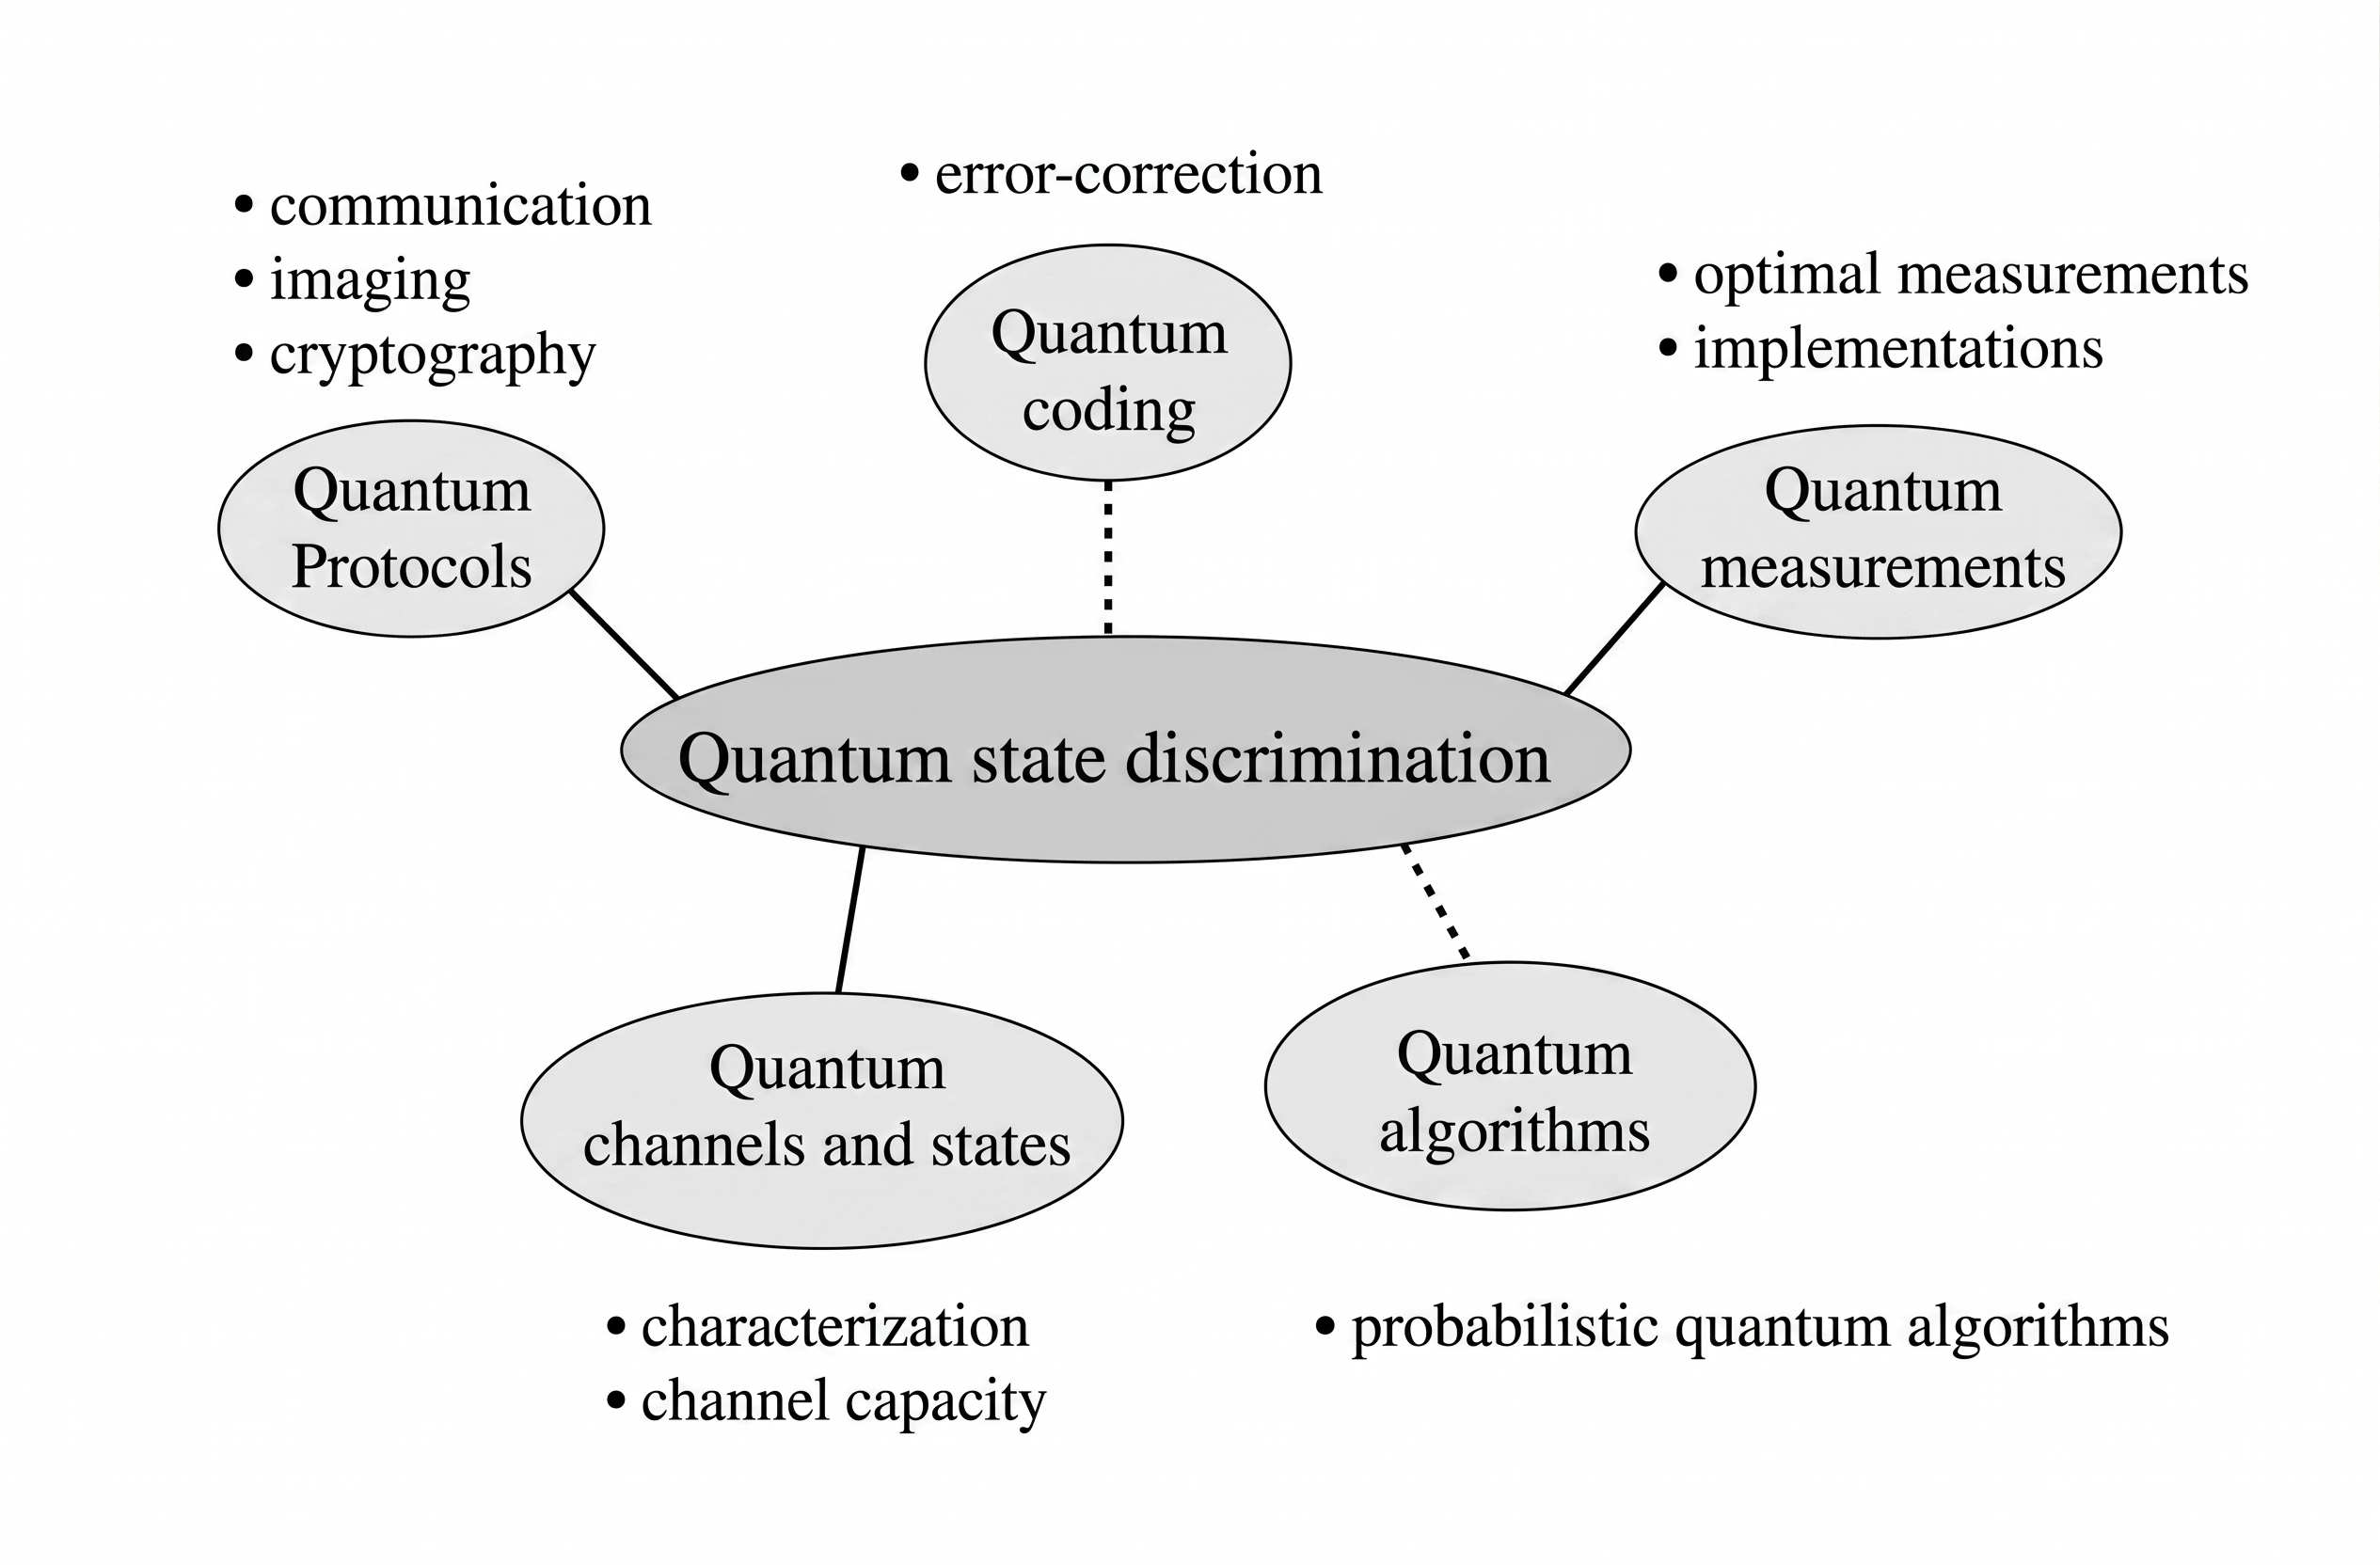
\includegraphics[width=1.0\textwidth]{figures/qsd.jpg}
    \caption{An overview of the central role of quantum state discrimination in quantum information theory.\cite{mainref}}
    \label{fig:qsd_overview}
\end{figure}

Quantum state discrimination lies at the heart of quantum computation and communication. The specific strategy of state discrimination applied depends on the task in quantum information theory to be solved. For example, using state discrimination techniques, we can show that quantum mechanics does not permit perfect discrimination between nonorthogonal states $|\psi_0\rangle$ and $|\psi_1\rangle$---a result that is also directly implied by the no-cloning theorem.\\

To demonstrate this, assume we have a POVM with two elements $\Pi_0$ and $\Pi_1$. For perfect discrimination, we require that

\begin{equation}
    \Pi_0 |\psi_1\rangle = 0
\end{equation}
\begin{equation}
\Pi_1 |\psi_0\rangle = 0
\end{equation}

This means that if outcome $0$ is obtained, we deduce the state was $|\psi_0\rangle$, and if outcome $1$ is obtained, we deduce the state was $|\psi_1\rangle$. The POVM operators must also satisfy the completeness relation

\begin{equation}
    \Pi_0 + \Pi_1 = \mathbb{I}
\end{equation}

To derive the necessary condition for perfect discrimination, we multiply the above equation on the left by $\langle\psi_0|$ and on the right by $|\psi_1\rangle$:

\begin{equation}
    \langle\psi_0| (\Pi_0 + \Pi_1) |\psi_1\rangle = \langle\psi_0| \mathbb{I} |\psi_1\rangle
\end{equation}

Distributing the left-hand side gives

\begin{equation}
    \langle\psi_0|\Pi_0|\psi_1\rangle + \langle\psi_0|\Pi_1|\psi_1\rangle = \langle\psi_0|\psi_1\rangle 
\end{equation}

Now, from the perfect discrimination conditions, we have $\Pi_0|\psi_1\rangle = 0$. Therefore, the first term $\langle\psi_0|\Pi_0|\psi_1\rangle = 0$. For the second term, note that $\Pi_1$ is a positive operator. If $\Pi_1|\psi_0\rangle = 0$, then taking the adjoint gives $\langle\psi_0|\Pi_1 = 0$. However, this does not directly imply $\langle\psi_0|\Pi_1|\psi_1\rangle = 0$. In standard unambiguous discrimination, the POVM elements are constructed such that $\Pi_1$ projects onto a subspace orthogonal to $|\psi_0\rangle$, which indeed forces $\langle\psi_0|\Pi_1|\psi_1\rangle = 0$. Under this construction, we have,

\begin{equation}
    0 + 0 = \langle\psi_0|\psi_1\rangle
\end{equation}

Thus,

\begin{equation}
    \langle\psi_0|\psi_1\rangle = 0 
\end{equation}

This condition can only be satisfied if the states $|\psi_0\rangle$ and $|\psi_1\rangle$ are orthogonal. Consequently, perfect discrimination is impossible for non-orthogonal states. Insights such as these are prevalent when applying state discrimination to problems in quantum information theory. The fact that we cannot perfectly distinguish between non-orthogonal states is what makes quantum key distribution possible.\\

Another important use of state discrimination is to characterize properties of quantum states, such as entanglement and separability. Much research has been devoted to this area. One of the main motivations behind such studies is to determine whether entangled states are useful for certain tasks, or whether entanglement is needed for a given task at all. Quantum metrology, quantum imaging, and the classical capacity of quantum channels are examples of such investigations.\\

State discrimination is also indispensable in quantum error correction. Error correction cannot be performed without syndrome measurement. A syndrome measurement determines whether a quantum state has been corrupted and, if so, which part of the state has been affected. The syndrome measurement is typically a multi-state measurement that does not disturb the encoded state but still provides information about the error. Such measurements lie at the heart of error correction.\\

Finally, state discrimination has found uses in quantum algorithms through a variant known as quantum state filtering. In quantum state filtering, the goal is to determine whether an unknown quantum state is a specific state $|\psi_k\rangle$ from a set of known states $\{|\psi_1\rangle, \ldots, |\psi_N\rangle\}$, or one of the others. Using optimal solutions in quantum state filtering, it is possible to implement an efficient probabilistic quantum algorithm that distinguishes between sets of Boolean functions, which generalizes the Deutsch-Jozsa algorithm. It has also been proposed that quantum decision problems can be characterized by state discrimination.\\

Having discussed the role of state discrimination in the major topics of quantum information theory, we now introduce the encoding of information onto continuous variable states.

\subsection{Continuous Variables in Quantum Mechanics}
While quantum information is primarily concerned with discrete quantum variables, such as qubits, continuous variable states have always played an important role in quantum mechanics. The position and momentum of the quantized harmonic oscillator are continuous variables. Because a mode of the electromagnetic field can be thought of as a harmonic oscillator, its quadrature amplitudes (the electric and magnetic fields) are continuous variables. Due to this connection to the quantized electromagnetic field, the development of the laser in the 1960s inspired considerable research into the properties of continuous quantum variables.\\

Continuous variables also play an important role in quantum information. The original EPR thought experiment was formulated in terms of the entangled momentum and position states of two particles. Furthermore, one of the first experimental demonstrations of quantum teleportation was performed using continuous variable states. Many aspects of discrete quantum information theory have continuous analogues, including quantum codes. It is even possible to formulate a theory of universal quantum computation over continuous variables by combining linear optical devices such as phase shifters and beamsplitters with nonlinear elements such as downconverters and parametric amplifiers.\\

The primary reason for developing a theory of quantum information over continuous variables is a practical one. Most communication channels involve the exchange of bosons (such as photons or phonons), which correspond to quantized harmonic oscillators. Accordingly, the theory of quantum information over continuous variables is essential for understanding the physical limits of communication. Moreover, many important sensing and measurement techniques, including microscopy and radar, rely on bosonic systems. Quantum information over continuous variables is the key to understanding the limits of sensing and measurement and for devising methods to attain those limits. With this motivation, this work explores the fundamental limits of quantum communication and sensing and introduces techniques to achieve them, beginning with a review of continuous variable quantum information theory in the following chapter.

\subsection{Scope of This Work}
This subsection lists the major research areas in continuous variable quantum computing and quantum information, and situate the contributions of this work within them.\\

Major areas of research include:

\begin{enumerate}
    \item \textbf{Channel Capacity of the Noisy, Lossy Bosonic Channel:} A fundamental question in quantum communication is: what is the maximum rate at which information can be sent down a bosonic channel in the presence of loss and noise? The capacity of a quantum channel $\mathcal{E}$ with inputs drawn from an ensemble of states $\hat{\rho}_k$ with probabilities $p_k$ is given by its Holevo quantity,

\begin{equation}
    \chi(\{p_k, \hat{\rho}_k\}) = S\left(\sum_k p_k \mathcal{E}(\hat{\rho}_k)\right) - \sum_k p_k S\left(\mathcal{E}(\hat{\rho}_k)\right),
\end{equation}

where $S(\hat{\rho})$ is the von Neumann entropy of the state $\hat{\rho}$. Maximizing this quantity over all possible ensembles, including entangled inputs across multiple uses of the channel, yields the channel capacity. This maximization is often difficult to perform. The capacity of the bosonic channel with linear loss is known and is attained by sending ensembles of coherent states down the channel. By contrast, the capacity of the bosonic channel with linear loss and thermal noise remains unknown, although it is conjectured to also be attained by sending ensembles of coherent states.

    \item \textbf{Minimum Output Entropy Conjecture:} The capacity of the bosonic channel with linear loss and thermal noise is indeed attained by coherent state inputs if the bosonic minimum output entropy conjecture holds. This conjecture states that a coherent-state input yields the output with the minimum von Neumann entropy for a bosonic channel with additive Gaussian noise. Proving or disproving the bosonic minimum output entropy conjecture is perhaps the most important open problem in continuous variable quantum information theory.

    \item \textbf{Optimal Measurements for Distinguishing Bosonic States:} Distinguishing quantum states is an important component of quantum information science. Key results, such as the no-cloning theorem, the quantum teleportation protocol, and more recently the Yuen no-go theorem, have their origins in problems of state discrimination. The Helstrom bound gives the minimum probability of error technique for discriminating between two quantum states. The quantum Chernoff bound is an upper bound to the Helstrom limit of multiple-copy binary state discrimination, which is asymptotically tight in the error exponent. While the measurement techniques for attaining the Helstrom bound are known in principle, devising experimentally practical measurement techniques for attaining the Helstrom bound is not known in general. Moreover, even when the channel capacity for a quantum channel is attained by product state (unentangled) inputs, the measurement required to attain the capacity is the entangling `pretty-good' measurement, which may be hard to perform in practice. For example, even though the channel capacity for the bosonic channel with linear loss is attained by coherent state inputs, practical decoding techniques that attain this bound are not currently known.

\end{enumerate}
